\section{Results}
\label{section:results}

In order to analyze the decay processes, we first discuss the energetic
accessibility of different decay channels and then present the corresponding
Auger-Meitner decay widths.
In Fig. \ref{fig:sdip} we present the computed
single and double ionization spectra
of strontium obtained by DC-ADC calculations. The main peaks of the
ionization
from the Sr$4p_{3/2}$ and the Sr$4p_{1/2}$ have single ionization potentials (SIPs)
of \unit[28.277]{eV} and \unit[29.402]{eV}, respectively. The experimental
values of \unit[28.21]{eV} and \unit[29.17]{eV} are very close and
varify the applicability
of the chosen method \cite{Schmitz76}.
They are characterized by pole-strengths, which in this implementation
is defined as
the sum of the absolute squares of the $1h$ coefficients
\cite{Trofimov05}, of 0.76 and 0.80
(see Table \ref{tab:widths}). We will at this point treat them as single
configurations and analyze them in detail later.
These two single ionization energies are higher
than only one double ionization potential (DIP) of \unit[16.430]{eV},
which is to \unit[99.7]{\%} characterized by the double ionization from
the $5s$ valence. The Auger-Meitner process is therefore energetically accessible and
results in a single final state.
For radium the spectra are qualitatively the same and
lead to the same conclusion.

\begin{figure}[h]
 \centering
 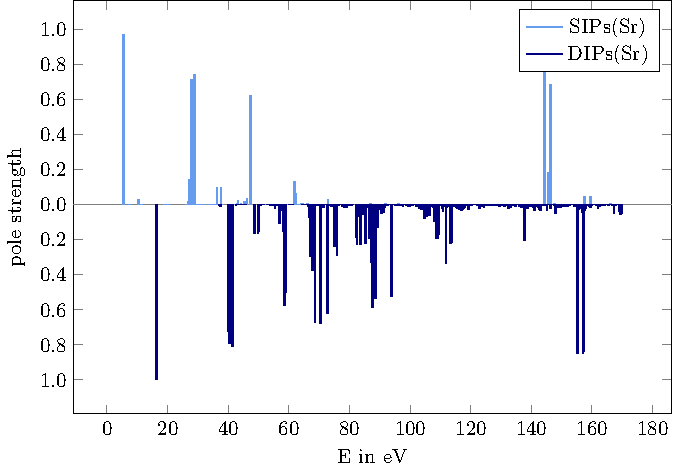
\includegraphics[width=\columnwidth]{pics/Sr_rel_sdip.pdf}
 \caption{Comparison of the single (SIP) and double (DIP) ionization spectra
          of the strontium obtained by a DC-ADC calculation.}
 \label{fig:sdip}
\end{figure}

\begin{table}[h]
 \centering
 \caption{}
 \begin{tabular}{lrrr}
  \toprule
   initial state    & energy $[\unit{eV}]$ & ps & $\Gamma [\unit{meV}]$\\
  \midrule
   Sr spinfree      & 28.599 & 0.78 &   0.56\\  
   Sr$4p_{1/2,1/2}$ & 29.402 & 0.80 &   0.10\\
   Sr$4p_{3/2,1/2}$ & 28.277 & 0.76 &   1.23\\
   Sr$4p_{3/2,3/2}$ & 28.277 & 0.76 &   1.17\\
%  \midrule
%   Ba$5p_{1/2,1/2}$ & 25.108 & 0.80 & unreliable\\
%   Ba$5p_{3/2,1/2}$ & 23.106 & 0.76 &   55.9\\
%   Ba$5p_{3/2,3/2}$ & 23.106 & 0.76 &   63.1\\
  \midrule
   Ra spinfree      & 21.836 & 0.49 &  28.56 \\  
   Ra$6p_{1/2,1/2}$ & 25.494 & 0.78 &   0.26\\
   Ra$6p_{3/2,1/2}$ & 19.267 & 0.50 &  93.16 \\
   Ra$6p_{3/2,3/2}$ & 19.267 & 0.50 &  98.86\\
  \bottomrule
 \end{tabular}
 \label{tab:widths}
\end{table}


We show the corresponding decay
widths of strontium and radium obtained by relativistic FanoADC-Stieltjes
calculations in Table \ref{tab:widths}
for the scalarrelativistic spinfree $(n-1)p^{-1}$ as well as the
fully relativistic $(n-1)p_{1/2,1/2}^{-1}$, $(n-1)p_{3/2,1/2}^{-1}$ and
$(n-1)p_{3/2,3/2}^{-1}$ initial states. They are illustrated in Fig. \ref{fig:gamma}.
To the best of my knowledge, the Auger-Meitner decay widths of these systems have
not been presented in the literature so far.
%, even though xyz compare their
%radiative lifetimes to Auger-Meitner widths, which they seem to have gained
%from private communication with xyz \cite{}.

Despite the difference in absolute numbers, the decay widths
of the different initial states show the same pattern. The decay width of
the $(n-1)p_{1/2,1/2}^{-1}$ initial state is lowest, while the decay widths
of the $(n-1)p_{3/2,1/2}^{-1}$ and
$(n-1)p_{3/2,3/2}^{-1}$ initial states are close and significantly higher than
for the $(n-1)p_{1/2,1/2}^{-1}$ initial state.
In case of the strontium atom, the decay width of the $p_{3/2}$ initial state
is approximately 12 times larger than the decay with of the $p_{1/2}$ initial state.
In radium, the corresponding factor is 380.
Furthermore, the decay width average of the $p_{3/2}$ initial state is increased 
by \unit[114]{\%} and \unit[236]{\%} for strontium and radium, respectively.
We can therefore observe an increase
of the decay width difference of the $p_{3/2}$ initial state both
compared to the $p_{1/2}$ and spinfree initial state for heavier atoms.
How can this result be understood?

\begin{figure}[h]
 \centering
 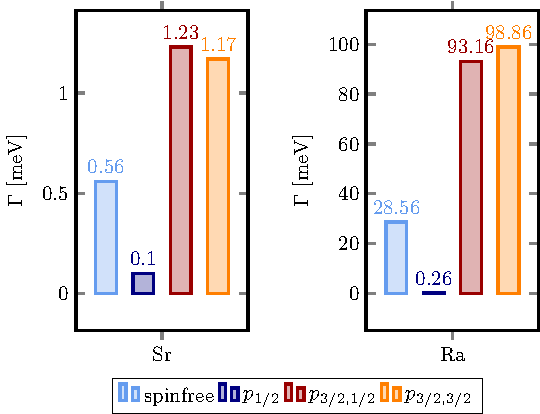
\includegraphics[width=0.95\columnwidth]{pics/gamma_group.pdf}
 \caption{Decay widths of strontium and radium after primary ionization from
          an $(n-1)p$ orbital obtained by relativistic FanoADC-Stieltjes
          calculations with different Hamiltonians. The spinfree Hamiltonian
          includes only scalarrelativistic effects, while the four-component
          DC Hamiltonian also includes spin-orbit coupling, which gives rise to
          three possible initial states: the $p_{1/2}^{-1}$ as well as the
          degenerate $p_{3/2,1/2}$ and $p_{3/2,3/2}$ initial state.
          The decay width of the $p_{1/2}$
          initial state is significantly lower than for either of the
          $p_{3/2}$ initial
          states.}
 \label{fig:gamma}
\end{figure}

Considering our previous findings about the role
of scalarrelativistic effects on electronic decay widths \cite{Fasshauer15_1},
we inspect the radial densities of the $(n-1)p$ and the $ns$ orbitals of the
strontium and radium ions,
which we assume to be involved in the decay process (see
Fig.~\ref{fig:radial_pure}).
In case of the strontium atom, the radial densities of the $4p_{1/2}$ and the
$4p_{3/2}$ orbitals are almost identical. But for the radium atom, the radial
density of the  $6p_{1/2}$ orbital is closer to the nucleus than
the radial density of the $6p_{3/2}$ orbital. This general property is already
visible in the analytic solutions of the one-electron system \cite{Bethe_Salpeter}.
Because the Auger-Meitner decay rates crucially depend on the overlap of the
involved orbitals, the decay widths of an $(n-1)p_{3/2}^{-1}$ initial state
can be expected to be higher than the decay widths of an $(n-1)p_{1/2}^{-1}$
initial state. These findings are reflected in the decay widths shown in
Fig.~\ref{fig:gamma} and Table \ref{tab:widths} and are consistent with the
observations of the noble gas Auger-Meitner processes in Ref. \cite{Fasshauer15_1}.


\begin{table}[h]
 \centering
 \caption{Radial expectation values $\langle r \rangle$ of
          orbitals involved in the Meitner process
          for different configurations
          given in {\AA}ngstr{\"o}m.
}
 \begin{tabular}{llrrrrr}
  \toprule
   $\langle r \rangle$ &     config. &   $(n-1)p_{1/2}$ & $(n-1)p_{3/2}$ & $(n-1)d_{3/2}$ & $(n-1)d_{5/2}$ & $ns_{1/2}$\\
  \midrule
   \multirow{2}{*}{Sr} & $4p^55s^2$ & 0.794 &     0.809    &      --        &        --      &  1.981\\
       &      $4p^54d5s$ &            0.802 &     0.818    &    1.332       &      1.375     &  2.062\\
   \multirow{2}{*}{Ra} & $6p^57s^2$ & 0.996 &     1.114    &      --        &        --      &  2.244\\
       &      $6p^56d7s$ &            1.001 &     1.120    &    1.768       &      1.821     &  2.290\\
  \bottomrule
 \end{tabular}
 \label{tab:widths}
\end{table}


\begin{figure}[h]
 \centering
 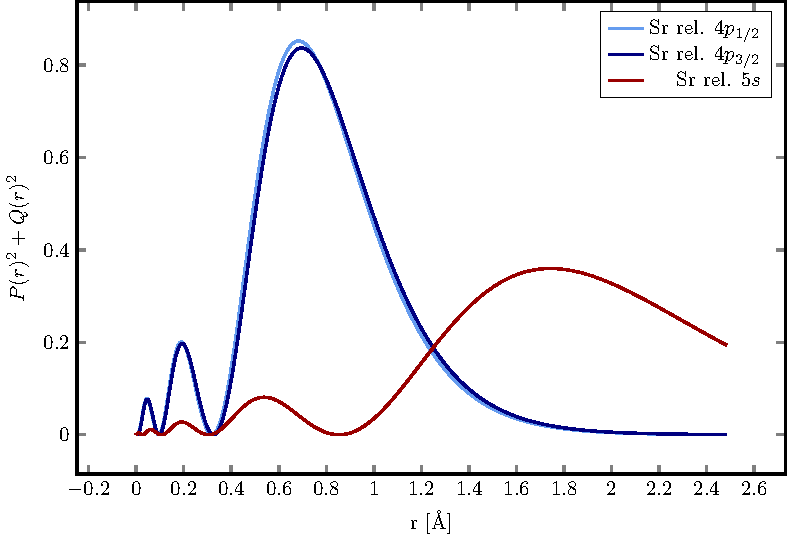
\includegraphics[width=\columnwidth]{pics/sr_ion_R.pdf}\\
 %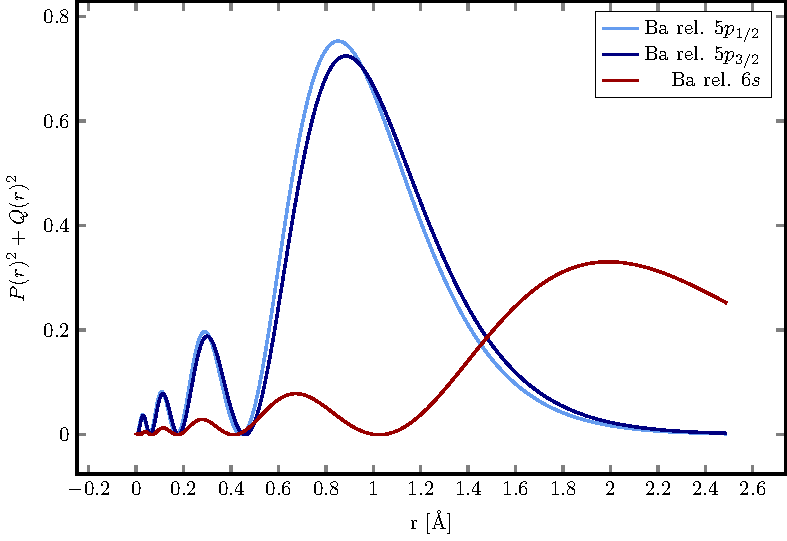
\includegraphics[width=\columnwidth]{pics/ba_ion_R.pdf}\\
 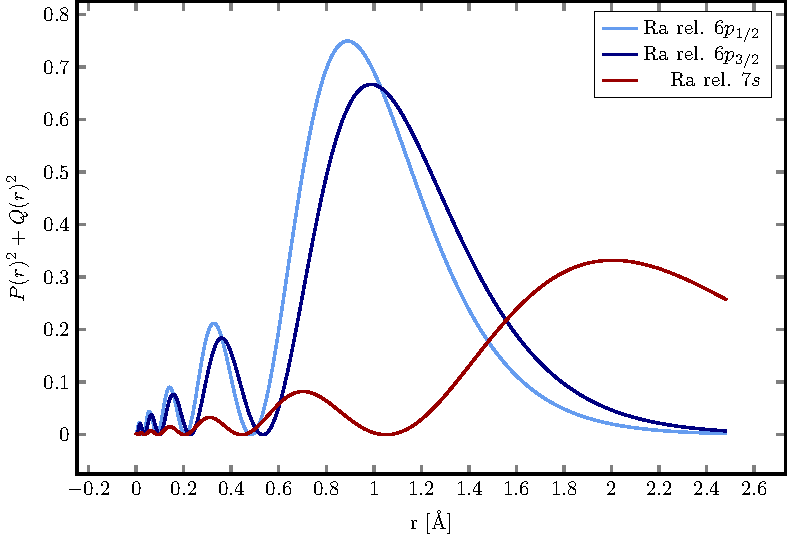
\includegraphics[width=\columnwidth]{pics/ra_ion_R.pdf}\\
 \caption{Radial densities of the orbitals of the $(n-1)p^5s^2$ ions
          involved in the Auger-Meitner decay.
          The expectation value of the electrons position of the $(n-1)p_{1/2}$
          orbital is lower than of the respective $(n-1)p_{3/2}$
          orbitals. The $ns$ orbitals of the ions experience a stronger
          contraction the those of the atom (not shown here).}
 \label{fig:radial_pure}
\end{figure}

However, the simulations of Auger-Meitner processes in other earthalkaline elements
have shown that correlation effects are important for the correct
description of these elements' decay widths. Both the investigations of
the Auger-Meitner process following primary ionization
from the $2p$ orbitals of calcium \cite{Nikkinen05}
as well as from the $4d$ orbitals of barium \cite{Rose80}
showed the necessity to include excitations from the valence $s$ orbital to
the $d$ orbitals, which are unpopulated in the ground state, in the
description of the initial state.
In our case, this would require to include the following configurations in our
simulations:
 $(n-1)p^{-1} \,ns^2$,
 $(n-1)p^{-1} \,(n-1)d \, ns$ and
 $(n-1)p^{-1} \,(n-1)d^2$ .    

Indeed, the analysis of the ADC eigenvectors of the initial states of both
strontium and radium showed
that beyond the single and main $1h$ contribution of the respective $p$ orbital, the
initial state is mainly characterized by $2h1p$ configurations of the
$(n-1)p^{-1} \,ns \, (n-1)d$ kind. They
are therefore automatically included in our simulations.
The FanoADC-Stieltjes approach is, however, limited
to second order perturbations in the wavefunction
and therefore does not go beyond $2h1p$ configurations. This means that the
$(n-1)p^{-1} \,(n-1)d^2$ configurations are not taken into account in this work.

How do these configurations affect the decay widths? Since the overlap of the
orbitals involved in the decay determine the decay widths, we show the
radial densities of the orbitals involved in the decay of the $6p^5 6d 7s$
configuration of radium in Fig.~\ref{fig:radial_ra}.
The $6p$ orbitals are slightly more contracted than in the $6p^{-1} \,7s^2$
configuration, while the $7s$ orbital is slightly decontracted by a difference
of the electron's distance from the nucleus $\Delta \langle r \rangle$
of \unit[0.046]{\AA}.
However, the $6d$ orbitals, which are involved
in the Auger-Meitner process of this configuration, show a large overlap with both
the $6p$ and the $7s$ orbitals. The corresponding decay width should therefore
be larger than the decay width of the $6p^{-1} \,7s^2$ configuration.
The prevalence of the $(n-1)p_{3/2}$ decay width over the $(n-1)p_{1/2}$
also holds for this configuration.
If the $(n-1)p^{-1} \,(n-1)d^2$ configurations
have non-negligible contributions,
the presented decay widths of Table~\ref{tab:widths} would be
lower bounds to the results of a more accurate decay width calculation.

\begin{figure}[h]
 \centering
 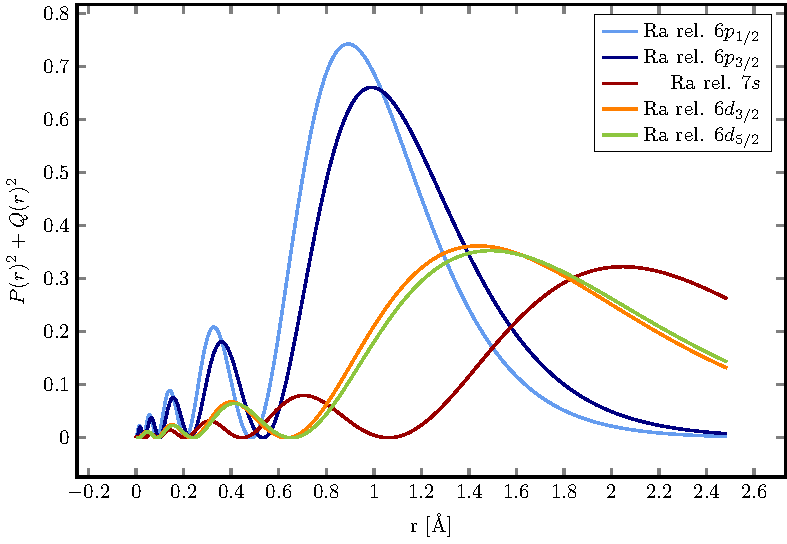
\includegraphics[width=\columnwidth]{pics/ra_6d_R.pdf}
 \caption{Radial densities of the radium orbitals of the ionic $6p^5 6d 7s$
          configuration involved in the Auger-Meitner decay. The overlap of the radial
          densities of the $6p$ orbitals with the radial densities of the $6d$ orbitals
          is more pronounced than with the radial density of the $7s$ orbital.}
 \label{fig:radial_ra}
\end{figure}

The observed differences in the decay widths for different initial states and
Hamiltonians can therefore not only be accounted for by relativistic
effects, but different contributions of the $(n-1)p^{-1} \,(n-1)d \, ns$
configurations may also affect the result.
In this case, the required measure of the $(n-1)p^{-1} \, ns^2$ configuration's
contribution to the ionized initial state is the pole-strength,
which are listed for the different initial states in Table \ref{tab:widths}.
The analysis of the eigenvectors has shown the other significant contributions
to be of the $(n-1)p^{-1} \,ns \, (n-1)d$ kind. We therefore assume that
they are the only other contributions and that their contribution is $1-\text{ps}$.
For strontium, the pole-strengths are similar but not identical for all initial
states and Hamiltonians. 
We can therefore predominantly attribute the decay width difference between the
$p_{3/2}$ and $p_{1/2}$ initial state to spin-orbit coupling rather than the
differences in the contributions of the $4p^54d5s$ configuration.
For radium, however, the pole-strengths of the initial states differ.
The $6p_{1/2}$ initial state has a pole-strength of 0.78, while both the
initial state of the scalarrelativistic Hamiltonian and the $6p_{3/2}$ initial
state have much lower pole-strengths of 0.49 and 0.50, respectively.
The $6p^{-1} \,7s^2$ configuration is therefore predominant for the $6p_{1/2}$
initial state, while it is not for the $6p_{3/2}$ initial state.
We can therefore not attribute the discrepancy of the decay widths of the
$6p_{1/2}$ and $6p_{3/2}$ initial states to spin-orbit splitting alone.
However, the initial state determined with the spinfree
Hamiltonian has a pole-strength comparable to the $6p_{3/2}$ initial states,
but the decay width of the $6p_{3/2}$ initial state is increased by \unit[236]{\%}
compared to the spinfree result and therefore
significantly lower.
Hence, we can explain the increase of the decay width from the spinfree to the
$6p_{3/2}$ initial state by spin-orbit coupling.

\begin{table}[h]
 \caption{Auger-Auger-Meitner (AM) decay widths and Coster-Kronig (CK) widths
          of $M_2$ and $M_3$ shells in \unit{eV} extracted from
          Ref. \cite{Chen81}.}
 \begin{tabular}{ccrrr}
 \toprule
 Z & Element & $\Gamma_\text{AM}(L_2)$ & $\Gamma_\text{AM+CK}(L_2)$ & $\Gamma_\text{AM}(L_3)$\\
 \midrule
 25 & Mn & 0.390 &  --   & 0.337 \\
 30 & Zn & 0.664 &  --   & 0.689 \\
 36 & Kr & 1.101 & 1.219 & 1.167 \\
 40 & Zr & 1.373 & 1.578 & 1.465 \\
 45 & Rh & 1.705 & 2.029 & 1.860 \\
 47 & Ag & 1.832 & 2.192 & 2.028 \\
 50 & Sn & 2.016 & 2.454 & 2.256 \\
 52 & Te & 2.128 & 2.614 & 2.406 \\
 54 & Xe & 2.236 & 2.767 & 2.557 \\
 56 & Ba & 2.336 & 2.912 & 2.696 \\
 60 & Nd & 2.456 & 3.060 & 2.897 \\
 63 & Eu & 2.534 & 3.146 & 3.041 \\
 67 & Ho & 2.611 & 3.233 & 3.211 \\
 70 & Yb & 2.662 & 3.285 & 3.340 \\
 74 & W  & 2.753 & 3.423 & 3.543 \\
 80 & Hg & 2.877 & 3.600 & 3.878 \\
 90 & Th & 3.060 & 3.877 & 4.464 \\
 92 & U  & 3.082 & 4.272 & 4.571 \\
 96 & Cm & 3.126 & 5.386 & 4.805 \\
 98 & Cf & 3.146 & 5.360 & 4.934 \\
100 & Fm & 3.168 & 5.586 & 5.060 \\
 \bottomrule
 \end{tabular}
 \label{tab:L}
\end{table}

\begin{table}[h]
 \caption{Auger-Auger-Meitner (AM) decay widths and Coster-Kronig (CK) widths
          of $M_2$ and $M_3$ shells in \unit{eV} extracted from
          Ref. \cite{Chen83}.}
 \begin{tabular}{ccrrrr}
 \toprule
 Z & Element & $\Gamma_\text{AM}(M_2)$ & $\Gamma_\text{AM+CK}(M_2)$ & $\Gamma_\text{AM}(M_3)$ & $\Gamma_\text{AM+CK}(M_3)$ \\
 \midrule
 67 & Ho &  0.687 &  9.484 & 0.977 &  9.823\\
 70 & Yb &  0.277 & 10.259 & 1.125 &  9.949 \\
 74 & W  &  0.839 & 11.870 & 1.342 & 10.529 \\
 78 & Pt &  1.257 & 13.148 & 1.569 &  9.735 \\
 80 & Hg &  1.313 & 13.580 & 1.673 & 10.166 \\
 85 & At &  1.403 & 13.597 & 1.990 & 10.879 \\
 88 & Ra &  1.634 & 14.169 & 2.170 & 10.667 \\
 90 & Th &  1.650 & 14.404 & 2.264 &  9.973 \\
 92 & U  &  1.727 & 14.557 & 2.375 & 10.235 \\
 95 & Am &  1.836 & 15.130 & 2.629 & 10.850 \\
 \bottomrule
 \end{tabular}
 \label{tab:M}
\end{table}

\begin{table*}[ht]
 \caption{Auger-Meitner (AM) decay widths and Coster-Kronig (CK) widths
          of $M_4$ and $M_5$ shells
          in \unit{eV} extracted from
          Ref. \cite{Chen80}.}
 \begin{tabular}{ccrrr}
 \toprule
 Z & Element & $\Gamma_\text{AM}(M_4)$ & $\Gamma_\text{AM+CK}(M_4)$ & $\Gamma_\text{AM}(M_5)$\\
 \midrule
 70 & Yb & 1.408 & 2.445 & 1.460 \\
 74 & W  & 1.758 & 1.831 & 1.830 \\
 80 & Hg & 2.259 & 2.381 & 2.452 \\
 83 & Bi & 2.512 & 2.670 & 2.753 \\
 88 & Ra & 2.923 & 3.126 & 3.253 \\
 92 & U  & 3.203 & 3.528 & 3.611 \\
 96 & Cm & 3.646 & 4.089 & 4.075 \\
100 & Fm & 4.000 & 4.488 & 4.583 \\
 \bottomrule
 \end{tabular}
 \label{tab:M45}
\end{table*}


Based on these consistent findings, we can formulate the following rule of thumb for
the relative Auger-Meitner decay widths:\\
Two ionized initial states that stem from the same non-relativistic configuration and
are split by spin-orbit coupling will have different decay widths, where the decay width
of the $l-\frac12$ initial state will be significantly lower than the decay width of
the $l + \frac12$ initial state.\\
In contrast to the effect imposed by scalarrelativistic effects, this rule
of thumb is independent of the angular moment quantum number $l$, because the
$l-\frac12$ will always be contracted more strongly than the corresponding
$l+\frac12$ orbital and the final state orbitals will be further away from
the nucleus than the initial state orbitals.

We can also expect this rule of thumbs to extent to ICD and
Electron Transfer Mediated Decay (ETMD) processes as well. The ICD
decay widths partly depend on the transition dipole moment between the
initial and final state of the initially ionized unit, which in return increases
with the overlap of the electron densities of the involved orbitals.
The ETMD decay widths are determind by the orbital overlap of two different units,
which is larger for orbitals further away from the nucleus.
Hence the same argumentation as for the Auger-Meitner process is valid in both
cases.

%We conclude that the spin-orbit coupling does affect
%the Auger-Meitner decay widths, even though it is not the only factor for the
%earth alkaline atoms.


